%!TEX ROOT=formularioFisica.tex

\section{Elettromagnetismo}
Il padre di questa branca della fisica è Maxwell e con le sue quattro equazioni descrive il campo
elettro-magnetico e riassume le precedenti teorie.
\subsection{Le equazioni di Maxwell}
\begin{alignat*}{2}
  \Phi_{S_{ch}}(\vec{E},t) &= \frac{\sum q_i}{\varepsilon_0} &\quad \Phi_{S_{ch}}(\vec{B},t)&=0\\
  C_\Gamma(\vec{E},t) &= -\frac{\Delta \Phi(\vec{B})}{\Delta t} & C_\Gamma(\vec{B},t) &=
  \mu_0 \left[ i+\varepsilon_0 \frac{\Delta\Phi(\vec{E})}{\Delta t} \right]
\end{alignat*}
Queste sono le equazioni viste come funzione, anche se più spesso vengono definite attraverso
integrali
\begin{alignat*}{2}
  \int_{S_{ch}}\vec{E}\cdot\dif\vec{S} &= \frac{\sum q_i}{\varepsilon_0} &\quad 
  \int_{S_{ch}}\vec{B}\cdot\dif\vec{S}&=0\\
  \oint_\Gamma\vec{E}\cdot\dif\vec{l}&=-\der{\Phi(\vec{B})}{t} & 
  \oint_\Gamma\vec{B}\cdot\dif\vec{l}&=
  \mu_0 \left[ i+\varepsilon_0 \der{\Phi(\vec{E})}{t} \right]
\end{alignat*}

Le prime due leggi erano già presenti nei campi statici (la prima sottoforma di Legge di Gauss). Le
seconde due invece sono ricavate attraverso esperimenti.

\subsection{La Terza legge di Maxwell}
La terza legge di Maxwell deriva dalla forza elettromotrice indotta. Se Faraday
ha trovato una forza elettromotrice indotta che produce la corrente, Maxwell va ancora più indietro
e l'unica cosa che può genera una forza elettromotrice è un \textbf{campo elettrico}.\\
Per andare a ricavare il campo elettrico, bisogna andare a ridefinire la forza
elettromotrice. Essa è il lavoro necessario a portare
l'unità di carica da un polo all'altro, diviso la carica. Quindi
\begin{equation*}
  \mathcal{E} = \frac{L_{+\to-}}{q}
\end{equation*}
Il lavoro però è definito come
\begin{equation*}
  \sum\limits^{n}_{i=1} \vec{F}\cdot\Delta\vec{l}_i = 
  \sum\limits^{n}_{i=1} \Delta q\vec{E}_i\cdot\vec{l}_i=
  \Delta q \sum\limits^{n}_{i=1} \vec{E}_i\cdot\vec{l}_i
\end{equation*}
Quindi ora possiamo riscrivere 
\begin{equation*}
  \mathcal{E}=\frac{\cancel{\Delta q}\sum\limits^{n}_{i=1}\vec{E}_i\cdot\vec{l}_i}{\cancel{\Delta q}}
  = C_\Gamma(\vec{E})
\end{equation*}
Ma se ora torniamo indietro, riscriviamo che
\begin{equation*}
  C_\Gamma(\vec{E}) = -\der{\Phi(\vec{B})}{t}
\end{equation*}
Nella definizione abbiamo utilizzato una somma. In realtà sarebbe il limite di una somma che quindi
definisce un integrale definito. Si riscrive generalmente
\begin{equation*}
  \oint_\Gamma\vec{E}\cdot\dif\vec{l} = -\der{\Phi(\vec{B})}{t}
\end{equation*}
Ed ecco la terza legge di Maxwell. Cosa ci dice però? Ci dice che se è presente una variazione di
flusso, si genera un campo elettrico perpendicolare a quello magnetico.
Immaginando una spira in un campo magnetico uniforme d'intensità variabile, immobile, la forza che 
agisce su di essa è
\begin{equation*}
  \vec{F} = q\vec{E}+q\vec{v}\times\vec{B}
\end{equation*}
ma essendo $\vec{v} = \vec{0}$ e quindi $q\vec{v}\times\vec{B} = 0$, dunque la forza che fa muovere
le cariche è pari a $q\cdot E_{ind}$. Se l'intensità di $\vec{B}$ varia, le linee di forza di 
$\vec{E}$ sono orientate in modo definito dalla legge di Lenz.

\subsection{La Quarta legge di Maxwell}
La quarta legge parte dall studio di un circuito RC in continua e analizzato il
transitorio, Maxwell è andato a guardare la circuitazione tra le armature del condensatore.
La circuitazione calcolata prima dell'armatura è pari a
\begin{equation*}
  C_{\mathcolor{blue}{\Gamma_1}}(\vec{B}) = \mu_0\cdot i
\end{equation*}
dove $\mathcolor{blue}{\Gamma_1}$ è una linea chiusa attorno al filo conduttore. Se ora invece si 
prende una linea  $\mathcolor{red}{\Gamma_2}$ che passi attraverso le armature, la circuitazione sarà
\begin{equation*}
  C_{\mathcolor{red}{\Gamma_2}}(\vec{B}) = 0
\end{equation*}
in quanto non c'è corrente all'interno.
\begin{center}
  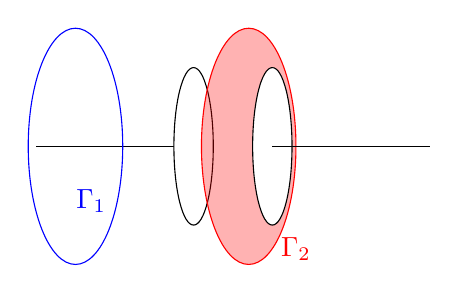
\begin{tikzpicture}
    \draw (0,0) -- (2,0);
    \draw[blue] (0.5,0) ellipse (0.6 and 1.5);
    \node[blue] at (0.7,-0.7) {$\Gamma_1$};
    \node[red] at (3.3,-1.3) {$\Gamma_2$};
    \filldraw[white,draw=black] (2,0) ellipse (0.25 and 1);
    \filldraw[fill opacity=0.3,red] (2.7,0) ellipse (0.6 and 1.5); 
    \filldraw[white,draw=black] (3,0) ellipse (0.25 and 1);
    \draw (3,0) -- (5,0);
  \end{tikzpicture}
\end{center}
Come si può capire però le due circuitazioni devono essere uguali. Maxwell per spiegare questo 
fenomeno, calcola il flusso del
campo elettrico su di una superficie $S$ circolare che ha come contorno la linea 
$\mathcolor{red}{\Gamma_2}$ possiamo calcolare semplicemente il flusso
\begin{equation*}
  \Delta\Phi(\vec{E}) = S \left[ \vec{E}(t+\Delta t)-\vec{E}(t) \right]
\end{equation*}
Sapendo che in un condensatore
\begin{equation*}
  E = \frac{\sigma}{\varepsilon_0} = \frac{q}{\varepsilon_0 S}
\end{equation*}
All'istante $t$, abbiamo una carica $q(t)$. All'istante $t+\Delta t$ invece abbiamo carica 
$q(t+\Delta t)$. Ma come possiamo riscriverla? Sapendo che
\begin{equation*}
  \Delta q = i\Delta t
\end{equation*}
e quindi 
\begin{equation*}
  q(t+\Delta t) = q(t) + i\Delta t
\end{equation*}
Avendo queste informazioni possiamo sostituirle nella formula del flusso di prima
\begin{equation*}
  \Delta\Phi(\vec{E}) = \left[ \frac{q+i\Delta t}{\varepsilon_0 S}-\frac{q}{\varepsilon_0 S} \right]
\end{equation*}
Semplificando otteniamo
\begin{equation*}
  \Delta\Phi(\vec{E}) = \frac{i\Delta t}{\varepsilon_0}
\end{equation*}
Abbiamo così trovato il termine mancante, una corrente mai rilevata prima.
\begin{equation*}
  i_s = \varepsilon_0\frac{\Delta\Phi(\vec{E})}{\Delta t}
\end{equation*}
Questa è definita \textbf{corrente di spostamento}.\\
Tornando al problema originale, la circuitazione diventa quindi
\begin{equation*}
  \oint_\Gamma \vec{B}\cdot\dif\vec{l} = \mu_0 \left( i+\varepsilon_0\der{\Phi(\vec{E})}{t} \right)
\end{equation*}
